% !TeX root = proyecto.tex

\cdtInstrucciones{En esta sección describa para cada máquina de estados y a que entidad corresponde. Utilice reglas ECA en el diagrama y elabore el diagrama de estados, una descripción del diagrama, una descripción de cada estado y una descripción de las acciones indicando que casos de uso están involucrados.}

% - - - - - - - - - - - - - - - - - - - - - - - - - - - - 
\subsection{Estados para un préstamo}

En la figura~\ref{fig:edos-prestamo} se muestran ...

\begin{figure}[htbp]
	\begin{center}
		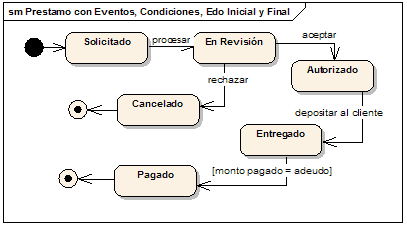
\includegraphics[width=.7\textwidth]{images/edoPrestamo}
		\caption{Máquina de estados de un Préstamo.}
		\label{fig:edos-prestamo}
	\end{center}
\end{figure}

\subsubsection{Estados}

\begin{description}
	\item[Estado:] Descripción del estado.
	\item[...] ...
\end{description}


\subsubsection{Acciones}

\begin{description}
	\item[Acción:] Descripción de la acción indicando el Caso de uso involucrado.
	\item[...] ...
\end{description}
